\section{IoTeX: panoramica su architettura e design}

\subsection{Principio di progettazione}
IoTeX mira a diventare la spina dorsale ed il sistema nervoso scalabile e incentrato sulla privacy dedicato all'IoT. Per raggiungere questo obiettivo e affrontare le sfide citate, la nostra architettura il design della nostra architettura è basato sui seguenti princìpi.

\subsubsection{Separazione delle responsabilità}
Connettere direttamente tutti i nodi IoT in una singola blockchain è un sogno che non può essere realizzato. Oltre al fatto che le diverse applicazioni IoT richiedono fondamentalmente diversi insiemi di funzionalità della blockchain, ospitare ogni nodo IoT sulla stessa blockchain la farebbe crescere rapidamente in dimensioni e richiesta computazionale, e alla fine diventerebbe troppo pesante per molti Dispositivi IoT. Invece, una separazione delle funzioni assicura che ogni blockchain interagisca con un gruppo specifico di nodi IoT e, allo stesso tempo, interagisca con altre blockchain quando necessario. Analogamente a quanto accade per Internet, dispositivi eterogenei prima formano un gruppo interconnesso, la intranet; intranet più piccole possono ulteriormente formare una intranet più grande, che alla fine si connette alla spina dorsale di internet e comunicano l'un l'altro.
La "Separazione delle responsabilità" di solito crea un sistema ben bilanciato per massimizzare sia l'efficienza che la privacy.

\subsubsection{Il Rasoio di Occam}
Diverse blockchain hanno utilizzi e applicazioni diverse, e dovrebbero essere progettate e ottimizzate verso direzioni diverse. Ad esempio, una blockchain dedicata all'inoltro delle transazioni tra le sue subchain non necessita su di essa vengano eseguiti smart-contract Turing-Completi; un'altra blockchain che colleghi dispositivi appartenenti alla stessa zona di fiducia non dovrebbe preoccuparsi troppo della privacy transazionale.

\subsubsection{IoT amichevole}
Come già detto, il mondo IoT è pieno di sistemi e nodi eterogenei, più o meno potenti in termini di risorse di calcolo, archiviazione e potenza. Dal momento che le operazioni che possono essere eseguite dai nodi deboli possono anche essere facilmente eseguite da quelli forti, le operazioni sulla blockchain dovrebbero essere progettate e ottimizzate per i nodi deboli, ovvero le operazioni dovrebbero essere abbastanza leggere da risparmiare risorse come potenza di calcolo, spazio di archiviazione ed energia.


\subsection{Architettura: Blockchain in Blockchain}
IoTeX è una rete di molte blockchain disposte gerarchicamente, dove le blockchain possono funzionare contemporaneamente tra loro mantenendo l'interoperabilità. Nel mondo IoTeX, come mostrato nella Figura \ref{fig:fig1}, la blockchain radice (\emph{rootchain}) gestisce molte blockchain indipendenti, o \emph{subchain}. Una subchain si connette e interagisce con quei dispositivi IoT con i quali ha qualcosa in comune, ad esempio hanno uno scopo funzionale simile, operano in
ambienti simili, o condividono un livello di fiducia simile. Se una subchain non funziona bene, ad esempio se viene attaccata o si verificano bug del software, la rootchain rimane completamente inalterata. Inoltre, sono supportate transazioni tra blockchain per trasferire valore e dati dalle subchain alla rootchain, oppure tra una subchain e l'altra attraverso la rootchain.

\begin{figure}[ht]
	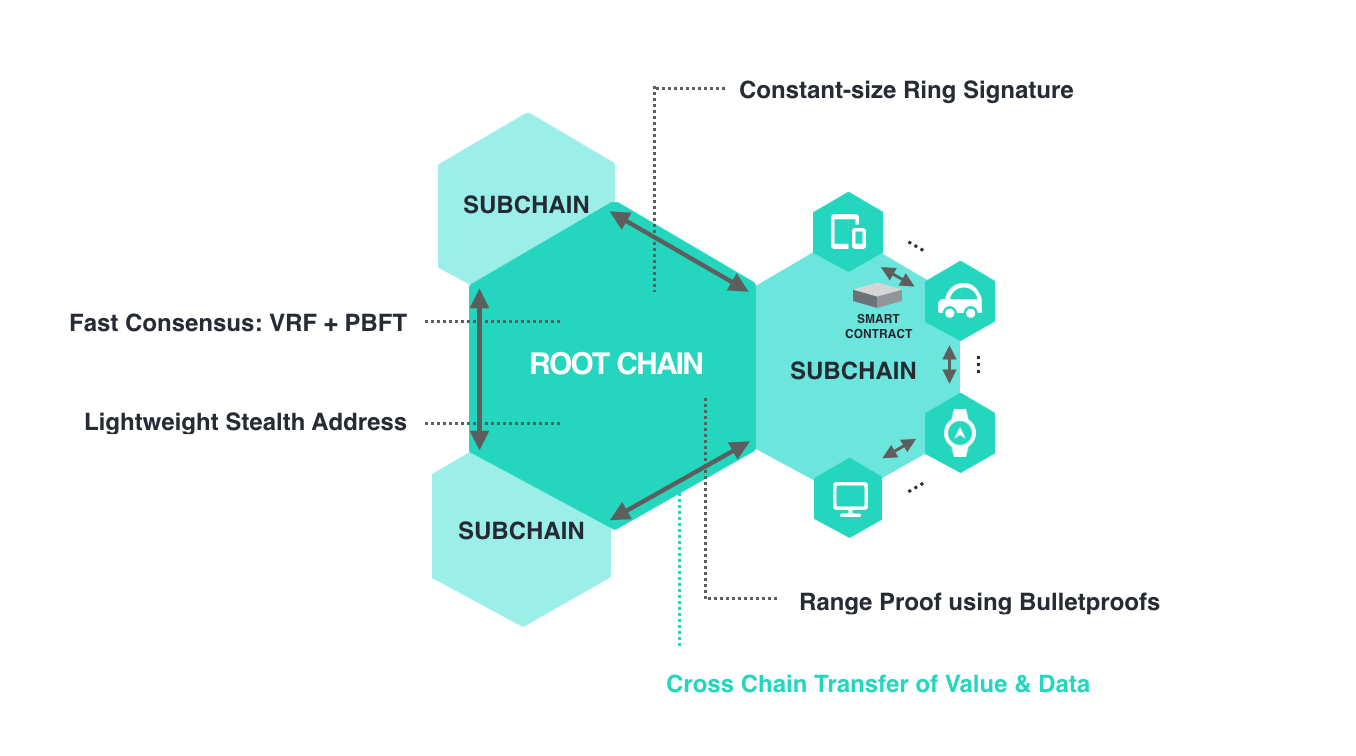
\includegraphics[width=\textwidth]{Figura1.png}
	\label{fig:fig1}
	\caption{IoTeX: Blockchain in blockchain, una architettura di rootchain con subchain}
\end{figure}

La blockchain radice è una blockchain pubblica accessibile da chiunque, che ha tre obiettivi principali:

\begin{enumerate}
	\item
	      \textbf{Inoltro} di valore e dati tra le subchain in modo da preservare la privacy per abilitare l'interoperabilità tra le subchain;
	\item
	      \textbf{Supervisione} delle subchain, ad esempio penalizzare gli operatori di subchain confiscando il deposito;
	\item
	      \textbf{Regolamento e ancoraggio} dei pagamenti e della fiducia per le subchain.
\end{enumerate}
Con questi obiettivi definiti, la rootchain si concentra in particolare su scalabilità, robustezza,
funzioni per preservare la privacy e capacità di controllare le subchain.
Una subchain, d'altra parte, potrebbe potenzialmente essere una blockchain privata e dipendere dalla rootchain per l'interazione con altre sottocatene. Una subchain richiede flessibilità
ed estendibilità per adattarsi ai diversi requisiti delle diverse applicazioni IoT. Una subchain sarà molto probabilmente gestita da operatori il cui ruolo è subordinato a un deposito di garanzia sufficiente, depositato sulla rootchain. Opzionalmente, il sistema consente agli operatori di nominare uno o più operatori che agiscono per suo conto, con o senza vincoli extra. L'operatore agisce come un client leggero nella rootchain, e come un nodo completo nella subchain per
confermare nuovi blocchi.
Nel complesso, le proprietà di rootchain e subchain sono riassunte in Tabella \ref{table:rootchainandsubchains}

\begin{table}[tp]%
	\caption{Confronto tra Rootchain e Subchain}
	\label{table:rootchainandsubchains}\centering %
	\begin{tabular}{l|l|l}
		\hline
		\textbf{Proprietà}          & \textbf{Rootchain}   & \textbf{Subchain}  \\
		\hline
		Pubblica vs Privata         & Pubblica             & Pubblica o Privata \\
		Scalabile                   & Necessario           & Varia              \\
		Robusta                     & Fortemente Richiesto & Richiesto          \\
		Incentrata sulla Privacy    & Richiesto            & Varia              \\
		Estendibilità               & Non-Turing completa  & Turing completa    \\
		Finalità Istantanea Blocchi & Richiesta            & Richiesta          \\
		\hline
	\end{tabular}
\end{table}

\subsection{Blockchain Root}
La blockchain root utilizza il modello basato su UXTO come Bitcoin \cite{c21} e Monero \cite{c20} per i seguenti motivi:

\begin{itemize}
	\item
	      L'ordinamento delle transazioni diventa banale, senza richiedere \emph{nonce} o
	      numeri di sequenza, il che pone richieste minime sugli schemi di consenso e permette di elaborare le transazioni in parallelo;
	\item
	      Applicando tecniche esistenti di conservazione della privacy come \emph{ring signature} e ZKSNARKs, diventa possibile nascondere il mittente, il destinatario e l'importo della transazione;
\end{itemize}

La blockchain radice è composta da blocchi collegati da hash, ed un blocco è costituito da  un'intestazione lo collega mediante un hash al blocco precedente, e da un elenco di transazioni.
La rootchain consente principalmente due tipi di transazione: (1) transazioni di base incluse
\texttt{P2PKH, P2SH, Multisig} e così via, e transazioni avanzate che consentono
operazioni tra blockchain come \texttt{BondedRegistration, Lock, ReLock, Reorg} ecc.. Le
transazioni validate vengono aggiunte ad un blocco che ha dimensione dinamica, con limite superiore di 8MB. Il nostro sistema di consenso produce un blocco ogni tre secondi come dettagliato
nella prossima sezione. La rootchain è progettata per essere non-Turning-Completa con il
supporto di uno script basato su stack e un ricco set di operazioni.

\subsection{Subchain}
IoTeX dispone di un framework per lo sviluppo e la fornitura di una subchain su misura
per applicazioni IoT decentralizzate incapsulando primitive a basso livello come il protocollo gossip
ed il meccanismo di consenso. Il modello di autorizzazione, le specifiche, i parametri,
e i tipi di transazione della subchain possono essere personalizzati per adattarsi alla sua applicazione.
Le subchain IoTeX utilizzano il modello basato sull'account, che è migliore per il tracciamento delle transizioni di stato.
Esistono due tipi di account, similmente a Ethereum, account regolari e
contratti. Le transazioni valide vengono aggiunte al blocco, che viene generato dallo stesso
schema di consenso della catena principale per raggiungere lo stesso livello di finality per rendere la comunicazione cross-chain più efficiente. Le subchain possono sia utilizzare il token della rootchain, IoTeX, oppure definire il proprio token. Il token definito dagli sviluppatori per le subchain possono essere distribuiti mediante vendita pubblica di token oppure scambiati sugli exchange pubblici.
Le subchain supportano smart contract, che vengono eseguiti su una macchina virtuale leggera ed efficiente. Attualmente stiamo valutando Web Assembly (WASM) \cite{c36}, uno standard Web emergente per la creazione di applicazioni Web ad alte prestazioni. WASM è veloce ed efficiente, può essere reso deterministico e dotato di sandbox a seguito di piccole modifiche così come tentato dal progetto EOS \cite{c9}. Anche altre opzioni vengono esplorate. Grazie agli smart contract, i dispositivi IoT collegati alla stessa subchain usano lo stato condiviso in due modi,

\begin{itemize}
	\item Innanzitutto, i dispositivi possono interagire con l'ambiente fisico in base agli stati delle loro subchain, ad es. le lampadine si accendono o spengono autonomamente in base allo stato di un orologio sulla stessa subchain;

	\item D'altra parte, i dispositivi possono cambiare il proprio stato sulla subchain quando
	      quando l'ambiente fisico cambia, ad esempio, il termostato aggiorna la temperatura tramite uno smart contract in base ai dati provenienti dal suo sensore;
\end{itemize}

\subsection{Comunicazione cross-blockchain}
Ci si aspetta che la comunicazione tra blockchain diverse sarà utilizzata di frequente nelle applicazioni in IoT. C'è sempre la necessità per un dispositivo IoT in una subchain di coordinarsi con un altro dispositivo in una diversa subchain. Ancora una volta, limitati dalla bassa potenza di calcolo e dal poco spazio di archiviazione dei dispositivi IoT, siamo motivati a progettare un tipo di comunicazione cross-blockchain che sia rapida ed economica in termini di risorse.

\subsubsection{Pegging e Finalità dei blocchi}
Il Pegging è un meccanismo per scalare la rete Bitcoin tramite \emph{"sidechain"}, originariamente
proposto in \cite{c1}. Esso si affida fortemente al \emph{Simplified Payment Verifcation} (SPV) \cite{c21}, e consente ai Bitcoin di \"spostarsi\" in modo efficiente dalla blockchain Bitcoin a una sidechain
e viceversa. L'idea alla base è semplice: i token vengono inviati ad un indirizzo speciale al fine di essere bloccati sulla blockchain Bitcoin; una volta confermata questa transazione di \texttt{Lock}, si invia la transazione \texttt{Reorg} alla sidechain, includendo la transazione \texttt{Lock} ed una
prova di inclusione (\emph{"Proof of inclusion"}), sotto forma di ramo Merkle. La sidechain usa SPV per verificare la transazione di \texttt{Reorg} e, se convalidata, crea una quantità di token equivalente e li invia all'indirizzo desiderato sulla sidechain. Ad oggi, il pegging funge da
primitiva per quasi tutti i protocolli di comunicazione cross-blockchain, ad es. Cosmos, Lisk,
Rootstock. Due flussi separati di pegging possono essere facilmente accoppiati insieme per creare il
cosiddetto Pegging a due vie (2WP) per renalizzare il trasferimento di token in entrambi i versi.

La finalità dei blocchi è la garanzia che ogni nuovo blocco generato sia "finale", e non può più essere
cambiato. La finalità dei blocchi ha un impatto sostanziale sull'attuazione concreta del pegging,
poiché è necessario aspettare fino a che la finalità di un blocco venga raggiunta (almeno con alta flessibilità) sulla blockchain da cui si invia prima di richiedere la \texttt{Reorg}. La maggior parte delle blockchain pubbliche come Bitcoin non hanno finalità istantanea. La blockchain ricevente può ottenere solo una assicurazione statistica, poiché man mano che più miners PoW confermano una transazione, aumenta la probabilità che essa sia stata accettata. Utilizzare un consenso con finalità risolve questo problema perché la blockchain ricevente ha la garanzia già con la conferma di un solo blocco sulla blockchain da cui si invia. Per le applicazioni IoT, il trasferimento tra le blockchain di valore e dati dovrebbe essere veloce e richiedere poche risorse, il che richiede un meccanismo di consenso con finalità sia sulla rootchain che sulle subchain. Il consenso IoTeX raggiunge la finalità istantanea dei blocchi, come dettagliato nella prossima sezione.

\subsubsection{Protocollo di comunicazione cross-blockchain}
Esaminiamo il protocollo ad un alto livello immaginando che un indirizzo di nome Charlie sulla
subchain 1 desideri inviare una transazione a un indirizzo chiamato David sulla subchain 2, e tutte e tre le blockchain usino lo stesso tipo di token, per semplicità senza costi di transazione. Si noti che applicando semplicemente il pegging, saranno necessarie quattro transazioni per effettuare una "remote call" dalla subchain 1 alla subchain 2 attraverso la rootchain, cioè, (1) una transazione di \texttt{Lock} sulla subchain 1; (2) una transazione di \texttt{Reorg} verso la rootchain; (3) un'altra transazione di \texttt{Lock} sulla rootchain; e (4) un'altra transazione di \texttt{Reorg} verso la subchain 2.
Questo processo indica che David deve attendere almeno 4 blocchi prima di accettare questa "remote call", e i dati che questa "remote call" trasporta devono essere archiviati su tutte e tre le blockchain, e ciò la rende lenta e costosa. Miriamo a ottimizzare questo processo combinando (2)
e (3) in un'unica transazione di \texttt{ReLock}, che non solo accelera l'intero processo ma
evita anche di archiviare i dati nella subchain 1 e nella rootchain. Il nostro protocollo è raffigurato
nella Figura \ref{fig:fig2}

\begin{figure}[ht]
	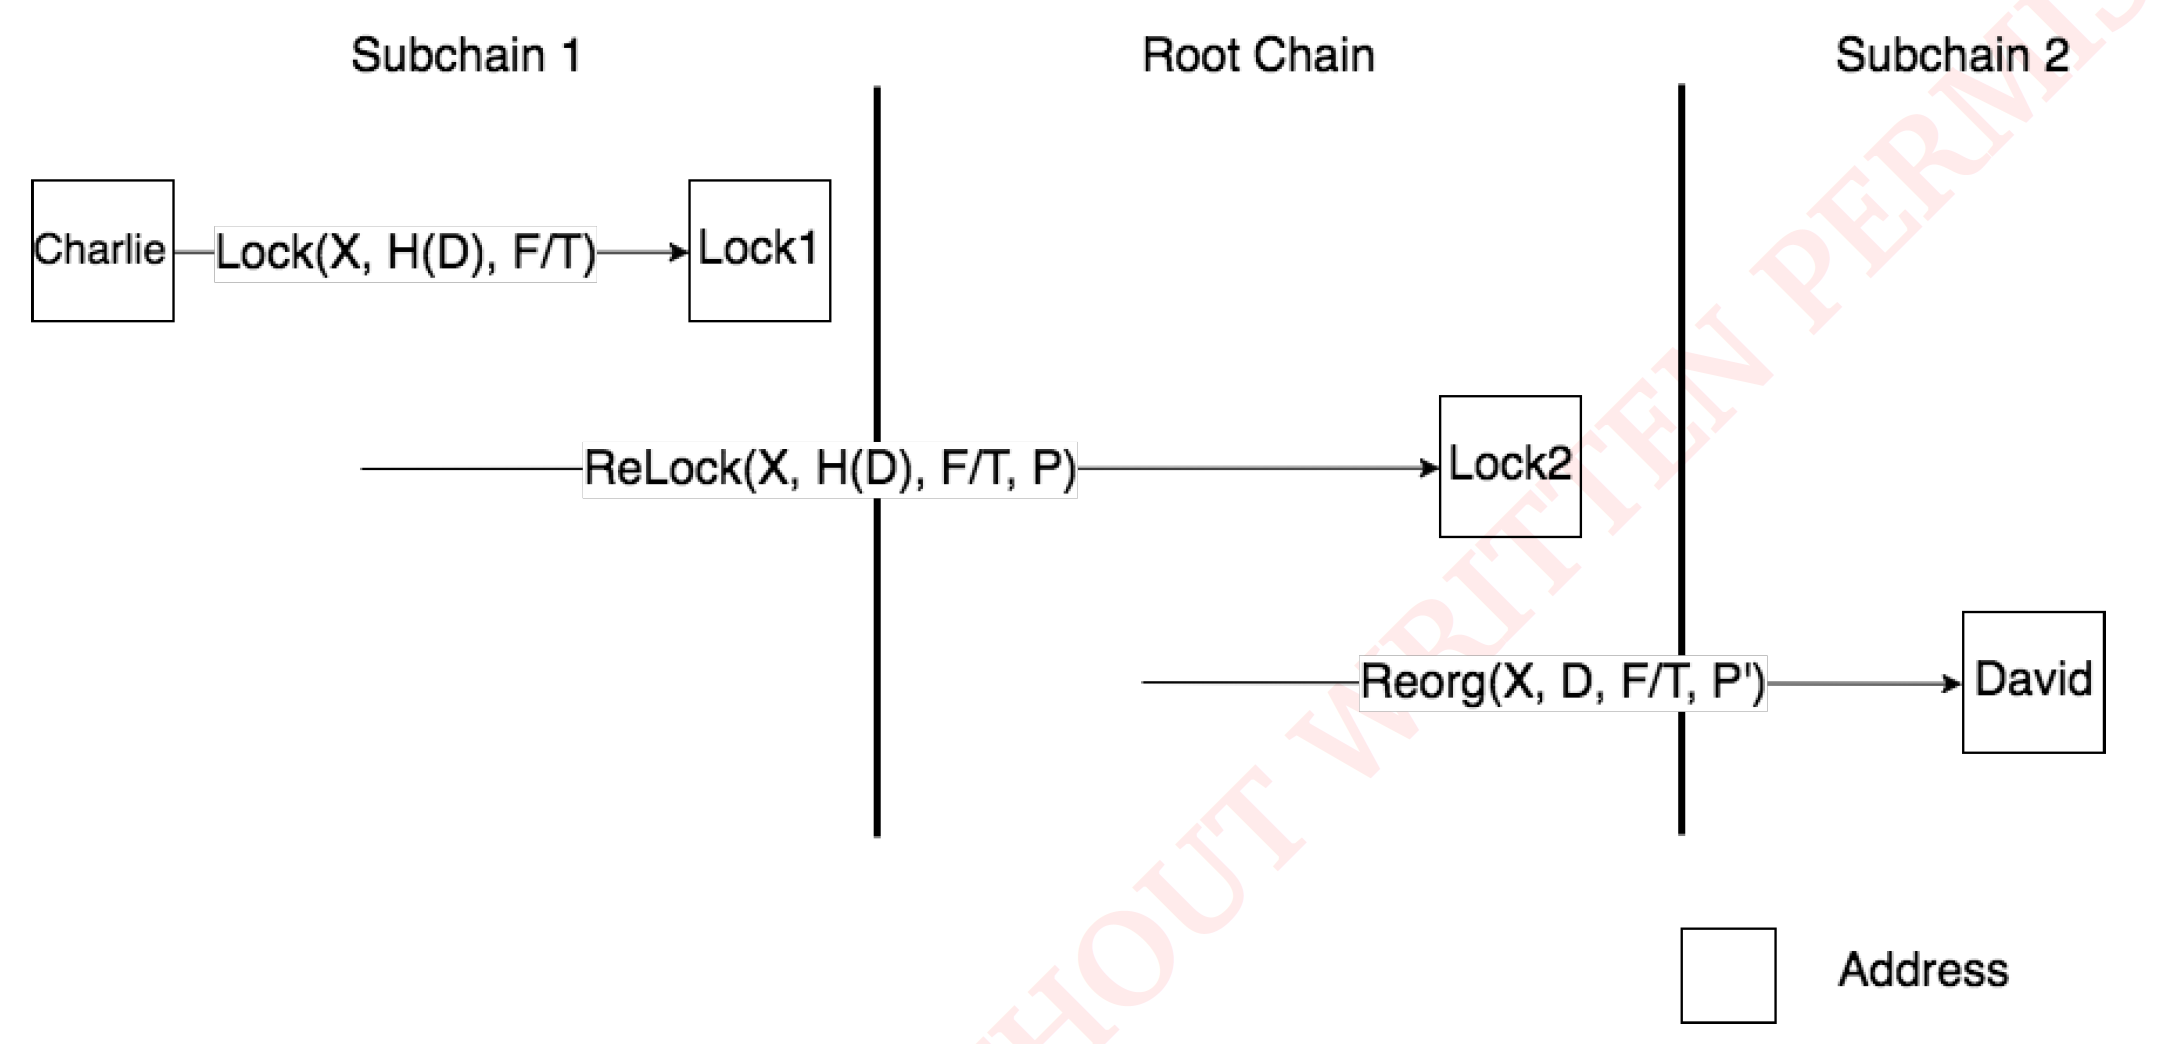
\includegraphics[width=\textwidth]{Figura2.png}
	\label{fig:fig2}
	\caption{Transazioni Cross-Bockchain}
\end{figure}

Il protocollo Cross-Blockchain di IoTeX è composto dai seguenti passi:

\begin{itemize}
	\item Ogni subchain viene registrate sulla rootchain inviando una transazione chiamata \texttt{BondedRegistration} alla rootchain, che include il nome della subchain, l'ID, la configurazione, il blocco "genesis", e la nomenclatura degli operatori; questo processo avviene una sola volta;

	\item Quando Charlie vuole inviare una transazione a David, inizia una transazione $\texttt{Lock}(X, H(D), F/T)$ dove $X$ è la quantità di token, $H(D)$ è l'hash dei dati $D$ da allegare, $F/T$ indica gli indirizzi sorgente e destinazione inclusi gli ID per entrambe le subchain;

	\item Una volta che la transazione di \texttt{Lock} è stata inclusa nella blockchain 1, Charlie inizia una transazione $\texttt{ReLock(X, H(D), F/T, S, P)}$ con la rootchain includendo $X, H(D), F/T$, alcune statistiche correnti della subchain 1 indicati con $S$ e una "\emph{proof-of-inclusion}" $P$ che comprende i rami Merkle delle intestazioni di blocchi recenti e rami Merkle che provano che la transazione \texttt{Lock} è stata inclusa;

	\item La rootchain valida la transazione \texttt{ReLock} e la accetta includendola nell'ultimo blocco, e crea $X$ token bloccandoli in un indirizzo speciale;

	\item Una volta che la transazione \texttt{ReLock} è stata inclusa nella rootchain, Charlie invia una transazione $\texttt{Reorg}(X, D, F/T, P')$ sulla rete della rootchain con $X, D, F/T$ ed un'altra \emph{proof-of-inclusion} $P'$ che prova l'inclusione della transazione \texttt{ReLock};

	\item Gli operatori della subchain 2 si accorgono della transazione \texttt{Reorg}, dunque validano e creano la stessa quantità di token sulla subchain 2 inviandoli all'indirizzo di David con associati i dati $D$.

\end{itemize}

\subsubsection{Condivisione della larghezza di banda della Blockchain Root}
Una possibile proeccupazione che riguarda la comunicazione cross-blockchain, è che subchain malevoli possano fare \emph{spam} sulla rootchain o un'altra subchain trasmettendo un'enorme quantità di transazioni cross-blockchain esaurendo la capacità dell'altra blockchain. Un modo di attenuare il problema è di lasciare che ogni subchain appalti la propria quota e limiti la frequenza delle transazioni da provenienti una subchain se la propria quota si esaurisce.

\begin{figure}[ht]
	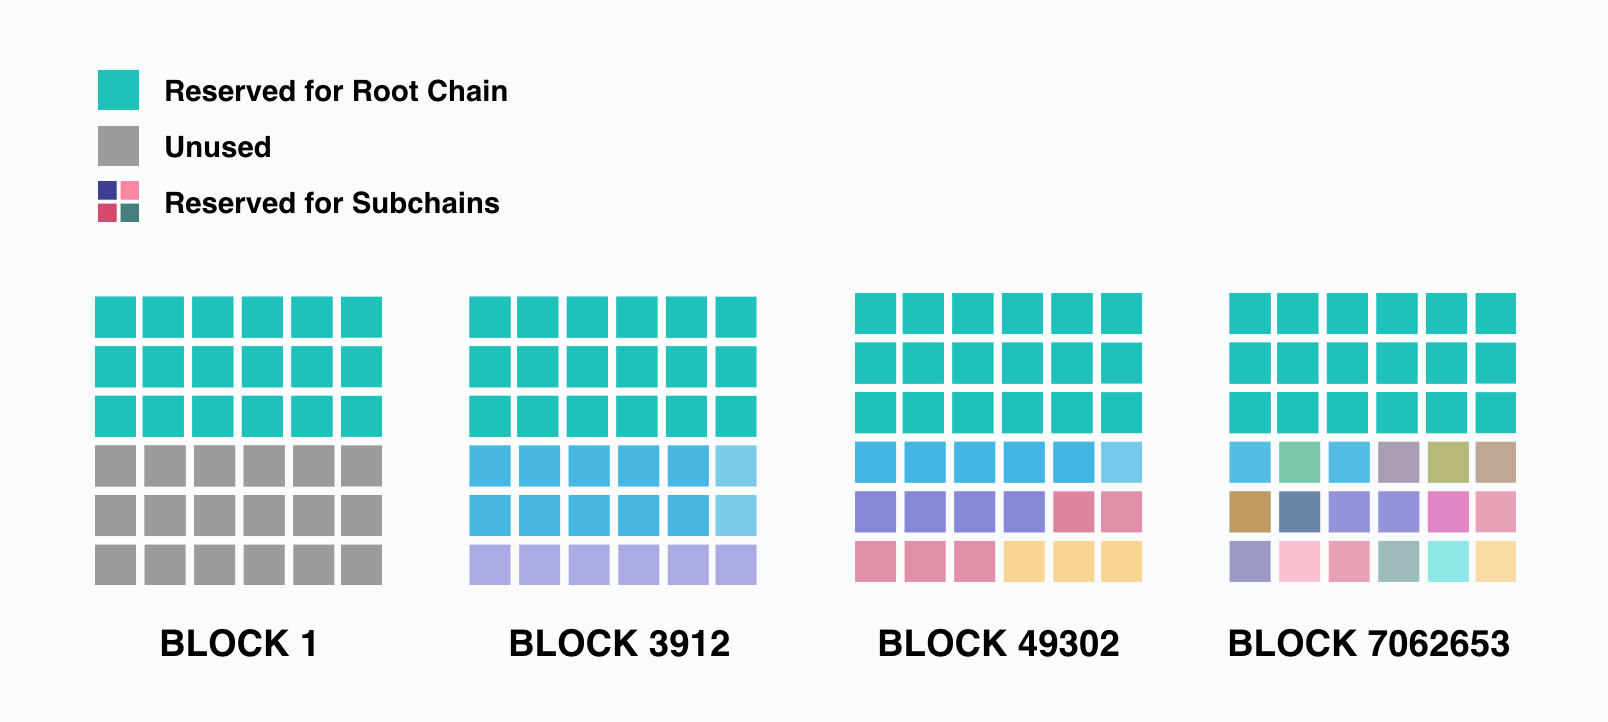
\includegraphics[width=\textwidth]{Figura3.png}
	\label{fig:fig3}
	\caption{Modello della Largezza di Banda per Sondividere la Capacità della Rootchain}
\end{figure}

Si potrebbe definire una quota basandosi sullo spazio all'interno di un blocco. Supponiamo che la dimensione massima di un blocco sia di 8MB, e che 4MB siano riservati per le normali transazioni all'interno della rootchain, e 4MB siano riservati per tutte le transazioni cross-blockchain, ulteriormente suddivisi in, diciamo 4096 parti di quota, con ogni parte di 1KB. Una subchain richiede l'allocazione $n$ parti di quota (con un limite massimo fissato) per gli usi desiderati, versando una cauzione proporzionale ad $n$. Ad ogni round, solo $n$KB possono essere occupati all'interno di ciascun blocco per le transazioni provenienti da quella subchain e per ognuna di esse viene scalata una "commissione di banda" dal deposito (per premiare i miner che aiutano ad applicare questa regola); le transazioni rimanenti vengono accodate e, alla fine, scartate quando scadono. L'allocazione delle quote può essere dinamica nel senso che subisce cambiamenti quando la rootchain cresce, come mostrato in Figura \ref{fig:fig3}. Se una subchain inviasse spam alle altre, consumerebbe il proprio deposito molto velocemente ed alla fine perderebbe la propria quata di banda. D'altra parte, se una subchain versasse un grosso deposito esclusivamente al fine di riservare una gran parte di larghezza di banda senza in realtà utilizzarla, la rootchain avrebbe un meccanismo per risarcire perte del deposito secondo il rapporto tra il numero medio di transazioni per blocco e la porzione di banda riservata, il che aiuta a stabilizzare la larghezza di banda riservata ad un valore vicino a quella attualmente utilizzata.